\documentclass[a4paper, 12pt]{extreport}

\usepackage[T2A]{fontenc}
\usepackage[utf8]{inputenc}
\usepackage[english,russian]{babel}
\usepackage{amssymb,amsfonts,amsmath,mathtext,cite,enumerate,float}
\usepackage{pgfplots}
\usepackage{graphicx}
\usepackage{tocloft}
\usepackage{listings}
\usepackage[table,xcdraw]{xcolor}
\usepackage{caption}
\usepackage{subcaption}
\usepackage{tempora}
\usepackage{adjustbox}
\usepackage{titlesec}
\usepackage{setspace}
\usepackage{geometry}
\usepackage{indentfirst}
\usepackage{pdfpages}
\usepackage{enumerate,letltxmacro}
\usepackage{threeparttable}
\usepackage[hidelinks]{hyperref}
\usepackage{flafter}
\usepackage{enumitem}
\usepackage{multirow}
\usepackage{ragged2e}

\usepackage[figure,table]{totalcount}
\usepackage{lastpage}

\setlist{nosep}

\newcommand{\ssr}[1]{\begin{center}
		\LARGE\bfseries{#1}
	\end{center} \addcontentsline{toc}{chapter}{#1}  }

\makeatletter
\renewcommand\LARGE{\@setfontsize\LARGE{22pt}{20}}
\renewcommand\Large{\@setfontsize\Large{20pt}{20}}
\renewcommand\large{\@setfontsize\large{16pt}{20}}
\makeatother
\RequirePackage{titlesec}
\titleformat{\chapter}[block]{\hspace{\parindent}\large\bfseries}{\thechapter}{0.5em}{\large\bfseries\raggedright}
\titleformat{name=\chapter,numberless}[block]{\hspace{\parindent}}{}{0pt}{\large\bfseries\centering}
\titleformat{\section}[block]{\hspace{\parindent}\large\bfseries}{\thesection}{0.5em}{\large\bfseries\raggedright}
\titleformat{\subsection}[block]{\hspace{\parindent}\large\bfseries}{\thesubsection}{0.5em}{\large\bfseries\raggedright}
\titleformat{\subsubsection}[block]{\hspace{\parindent}\large\bfseries}{\thesubsection}{0.5em}{\large\bfseries\raggedright}
\titlespacing{\chapter}{12.5mm}{-22pt}{10pt}
\titlespacing{\section}{12.5mm}{10pt}{10pt}
\titlespacing{\subsection}{12.5mm}{10pt}{10pt}
\titlespacing{\subsubsection}{12.5mm}{10pt}{10pt}

\makeatletter
\renewcommand{\@biblabel}[1]{#1.}
\makeatother

\geometry{left=30mm, right=10mm, top=20mm, bottom=20mm}

\onehalfspacing

\renewcommand{\theenumi}{\arabic{enumi}}
\renewcommand{\labelenumi}{\arabic{enumi}\text{)}}
\renewcommand{\theenumii}{.\arabic{enumii}}
\renewcommand{\labelenumii}{\asbuk{enumii}\text{)}}
\renewcommand{\theenumiii}{.\arabic{enumiii}}
\renewcommand{\labelenumiii}{\arabic{enumi}.\arabic{enumii}.\arabic{enumiii}.}

\renewcommand{\cftchapleader}{\cftdotfill{\cftdotsep}}

\addto\captionsrussian{\renewcommand{\figurename}{Рисунок}}
\DeclareCaptionLabelSeparator{dash}{~---~}
\captionsetup{labelsep=dash}

\captionsetup[figure]{justification=centering,labelsep=dash}
\captionsetup[table]{labelsep=dash,justification=raggedright,singlelinecheck=off}

\graphicspath{{images/}}

\newcommand{\floor}[1]{\lfloor #1 \rfloor}

\lstset{ %
	language=caml,                 
	basicstyle=\small\ttfamily, 
	numbers=none,               
	showspaces=false,            
	showstringspaces=false,      
	showtabs=false,             
	frame=single,              
	tabsize=2,                 
	captionpos=t,              
	breaklines=true,           
	breakatwhitespace=false, 
	escapeinside={\#*}{*)},   
	abovecaptionskip=-5pt
}

\pgfplotsset{width=0.85\linewidth, height=0.5\columnwidth}

\linespread{1.3}

\parindent=1.25cm

\def\labelitemi{---}
\setlist[itemize]{leftmargin=1.25cm, itemindent=0.65cm}
\setlist[enumerate]{leftmargin=1.25cm, itemindent=0.55cm}

\newcommand{\specialcell}[2][c]{%
	\begin{tabular}[#1]{@{}c@{}}#2\end{tabular}}

\frenchspacing

\begin{document}

% Титульная страница без нумерации
\begin{titlepage}
	\newgeometry{pdftex, left=2cm, right=2cm, top=2.5cm, bottom=2.5cm}
	\fontsize{12pt}{12pt}\selectfont
	\noindent \begin{minipage}{0.15\textwidth}
		
\includegraphics[width=\linewidth]{img/b_logo.png}
	\end{minipage}
	\noindent\begin{minipage}{0.9\textwidth}\centering
		\textbf{Министерство науки и высшего образования Российской Федерации}\\
		\textbf{Федеральное государственное бюджетное образовательное учреждение высшего образования}\\
		\textbf{«Московский государственный технический университет имени Н. Э.~Баумана}\\
		\textbf{(национальный исследовательский университет)»}\\
		\textbf{(МГТУ им. Н. Э.~Баумана)}
	\end{minipage}

	\noindent\rule{18cm}{3pt}
	\newline\newline
	\noindent ФАКУЛЬТЕТ $\underline{\text{«Информатика и системы управления»~~~~~~~~~~~~~~~~~~~~~~~~~~~~~~~~~~~~~~~~~~~~~~~~~~~~~~~}}$ \newline\newline
	\noindent КАФЕДРА $\underline{\text{«Программное обеспечение ЭВМ и информационные технологии»~~~~~~~~~~~~~~~~~~~~~~~}}$\newline\newline\newline\newline\newline\newline\newline

	\begin{center}
		\noindent\begin{minipage}{1.3\textwidth}\centering
		\Large\textbf{~~~Лабораторная работа №2}\newline
		\textbf{по дисциплине <<Анализ Алгоритмов>>}\newline\newline\newline
		\end{minipage}
	\end{center}

	\noindent\textbf{Тема} 			$\underline{\text{Алгоритм Винограда}}$\newline\newline
	\noindent\textbf{Студент} 		$\underline{\text{Платонова М. И.}}$\newline\newline
	\noindent\textbf{Группа} 		$\underline{\text{ИУ7-51Б}}$\newline\newline
	\noindent\textbf{Преподаватель} $\underline{\text{Волкова Л. Л.}}$\newline

	\begin{center}
		\vfill
		Москва~---~\the\year
		~г.
	\end{center}
	\restoregeometry
\end{titlepage}

\pagenumbering{arabic}
\setcounter{page}{2}

\def\contentsname{\begin{center}\MakeUppercase{СОДЕРЖАНИЕ}\end{center}}
\tableofcontents



\chapter*{ВВЕДЕНИЕ}
\addcontentsline{toc}{chapter}{ВВЕДЕНИЕ}

Матрицы находят широкое применение в различных областях, начиная от программирования и заканчивая физикой и экономикой. В математике матрица представляет собой таблицу чисел, организованную в строки и столбцы. Операции с матрицами, такие как сложение, умножение и возведение в степень, играют важную роль в решении различных задач.

Алгоритм Копперсмита~---~Винограда является одной из известных методик умножения квадратных матриц. Этот алгоритм был предложен Д. Копперсмитом и Ш. Виноградом, и он имеет наилучшую асимптотику среди известных алгоритмов умножения матриц. Однако на практике этот метод не всегда эффективен из-за высокой константы пропорциональности, что делает его предпочтительным только для матриц размером от $1000 \times 1000$, превосходящих возможности оперативной памяти большинства современных компьютеров.

Целью данной лабораторной работы является исследование алгоритмов умножения матриц (стандартный, классический и оптимизированный алгоритмы Винограда).

Для достижения поставленной цели необходимо решить следующие задачи:
\begin{itemize}
    \item[--] рассмотреть и реализовать классический алгоритм умножения матриц, алгоритм Винограда и его оптимизированную версию;
    \item[--] провести анализ временных затрат алгоритмов умножения матриц;
    \item[--] выполнить анализ трудоёмкости алгоритмов;
    \item[--] подготовить графики, отображающие результаты сравнительного анализа;
    \item[--] разработать набор тестов для оценки работоспособности реализованных алгоритмов;
    \item[--] сформулировать и представить результаты в отчёте о проведённой лабораторной работе.
\end{itemize}

\chapter{Аналитическая часть}
В этом разделе представлены алгоритмы стандартного умножения матриц, алгоритм Винограда и его оптимизированная версия~\cite{bib1}.

\section{Алгоритмы умножения матриц}

\subsection{Стандартный алгоритм}

Имеются две матрицы, $A$ и $B$, которые необходимо перемножить. Пусть $A$ имеет размерность \( M \times N \), а матрица $B$ — размерность \( N \times K \). Результирующая матрица $C$ будет иметь размерность \( M \times K \). Каждый элемент матрицы $C$ вычисляется по формуле (\ref{eq:VG}):

\begin{equation}
        \label{eq:VG}
	C_{ij} = \sum_{r=1}^{N} A_{ir} B_{rj}, \quad i \in \{1, \dots, M\}, \quad j \in \{1, \dots, K\}
\end{equation}

Стандартный алгоритм умножения матриц последовательно перемножает строки первой матрицы на столбцы второй, что позволяет получить элементы результирующей матрицы.

\subsection{Алгоритм Винограда}

Алгоритм Винограда -- это метод умножения квадратных матриц, предложенный в 1987 году Д. Копперсмитом и Ш. Виноградом. Основная идея -- уменьшить количество операций умножения для ускорения вычислений. 

Алгоритм Винограда использует предварительную обработку строк и столбцов матриц для ускорения вычислений. Вместо прямого вычисления скалярного произведения, алгоритм разбивает его на несколько простых частей, что позволяет сократить количество умножений. Имеются два вектора $V = (v_1, v_2, v_3, v_4)$ и $W = (w_1, w_2, w_3, w_4)$. Тогда их скалярное произведение рассчитывается по формуле (\ref{eq:VG2}):

\begin{equation}
    \label{eq:VG2}
	V \cdot W = v_1w_1 + v_2w_2 + v_3w_3 + v_4w_4.
\end{equation}

Алгоритм Винограда преобразует это выражение следующим образом (\ref{eq:VG3}):
\begin{equation}
	\label{eq:VG3}
	V \cdot W = (v_1 + w_2)(v_2 + w_1) + (v_3 + w_4)(v_4 + w_3) - v_1v_2 - v_3v_4 - w_1w_2 - w_3w_4.
\end{equation}

Данное выражение требует большего числа операций по сравнению с классическим методом, но оно позволяет проводить предварительные вычисления для строк и столбцов матриц, уменьшая количество операций умножения для каждого элемента произведения матриц.

\subsection{Оптимизированный алгоритм Винограда}
Оптимизированный алгоритм Винограда~\cite{bib2} предназначен для уменьшения количества операций умножения, что делает его более эффективным для работы с матрицами с матрицами размером от 
$500 \times 500$ и более. Идея оптимизации заключается в том, что предварительно рассчитанные значения для строк первой матрицы и столбцов второй сохраняются, что позволяет их повторно использовать. Это сокращает общие затраты на умножения и сложения.

В оптимизированном алгоритме для матрицы размером $n \times n$ выполняется $n^2$ сложений и $n^2/2$ умножений, что делает его быстрее по сравнению с классическим алгоритмом. Если размер матрицы нечётный, требуется дополнительное умножение для завершения расчётов.

Эта оптимизация существенно влияет на производительность при работе с большими матрицами, где снижение количества операций умножения позволяет сэкономить время и ресурсы.

\section*{Вывод}

В данном разделе рассмотрены стандартный алгоритм умножения матриц, алгоритм Винограда и его оптимизированная версия. Алгоритм Винограда отличается от классического тем, что предварительная обработка строк и столбцов позволяет уменьшить количество операций умножения. Оптимизированная версия алгоритма также сокращает количество умножений и увеличивает скорость работы при умножении матриц размером от $500 \times 500$ и более.


\chapter{Конструкторская часть}
В данном разделе представлены описания алгоритмов для умножения матриц, а также описание типов данных и оценка трудоёмкости реализованных алгоритмов.


\section{Описание структуры ПО}
На вход алгоритмов поступают две матрицы $matr1$ и $matr2$, размеры которых вводятся пользователем. Пользователь может выбрать один из двух вариантов ввода данных: вручную или сгенерировать случайные матрицы. На выходе программа возвращает результат произведения матриц, записанный в $res\_matr$.

\section{Описание алгоритмов}
Программа предоставляет выбор между тремя алгоритмами умножения матриц:
\begin{enumerate}
    \item[--] стандартный алгоритм умножения матриц;
    \item[--] умножение матриц по алгоритму Винограда;
    \item[--] оптимизированный алгоритм Винограда.
\end{enumerate}

\section{Алгоритм взаимодействия с пользователем}

Программа взаимодействует с пользователем через консольное меню:
\begin{itemize}
    \item[--] пользователь вводит размеры матриц;
    \item[--] программа предлагает выбрать способ ввода: вручную или случайная генерация матриц;
    \item[--] после ввода матриц пользователь может выбрать один из предложенных методов умножения.
\end{itemize}



Рисунки~\ref{fig:classic}~---~\ref{fig:win_22} представляют описание реализованных алгоритмов.
\clearpage

\begin{figure}[H]
    \centering
    \makebox[\textwidth][c]{\adjustbox{scale=0.8, center, right=20cm}{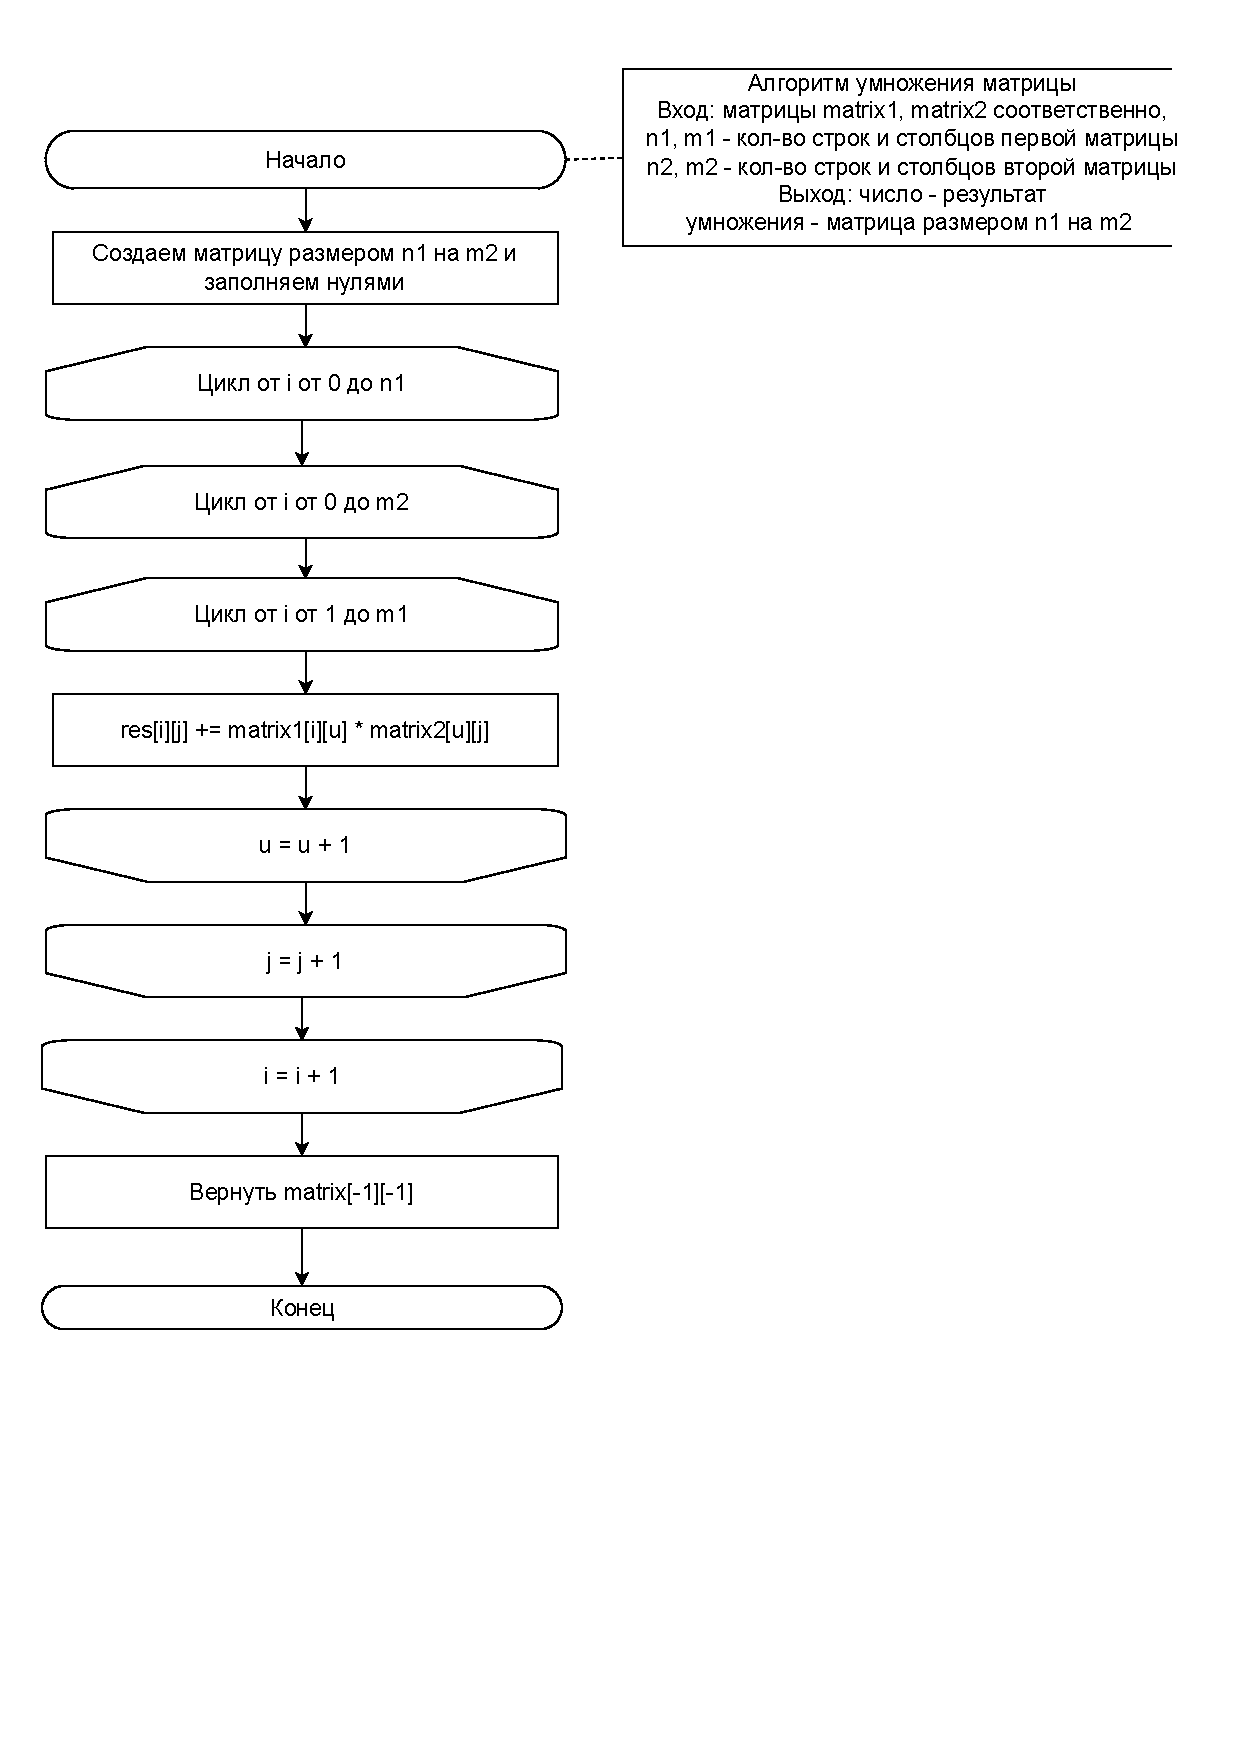
\includegraphics{img/classic.pdf}}}
    \caption{Стандартный алгоритм умножения матриц.}
    \label{fig:classic}
\end{figure}

\clearpage

\begin{figure}[H]
    \centering
    \adjustbox{scale=0.8, center}{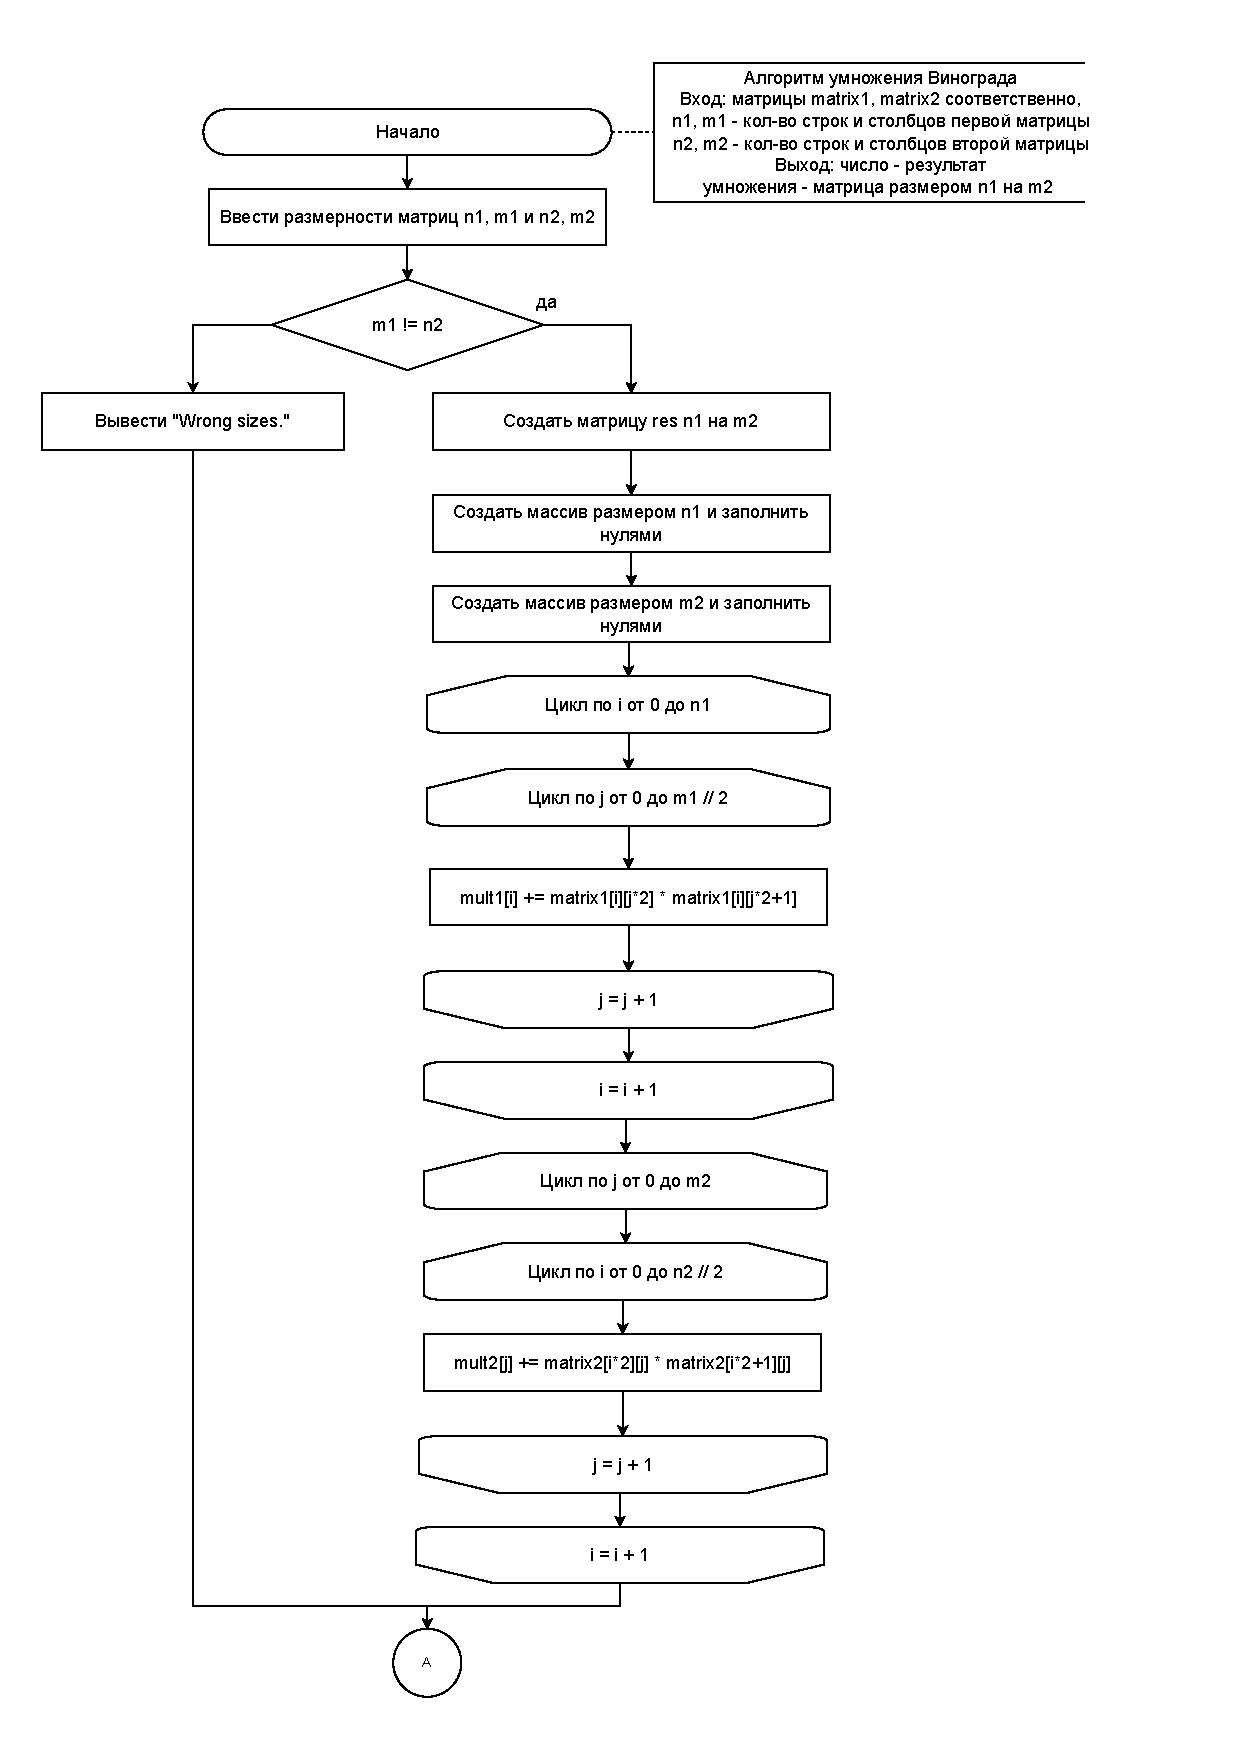
\includegraphics{img/win_11.pdf}}
    \caption{Алгоритм Винограда, часть 1.}
    \label{fig:win_11}
\end{figure}

\clearpage

\begin{figure}[H]
    \centering
    \adjustbox{scale=0.8, center, right=21cm}{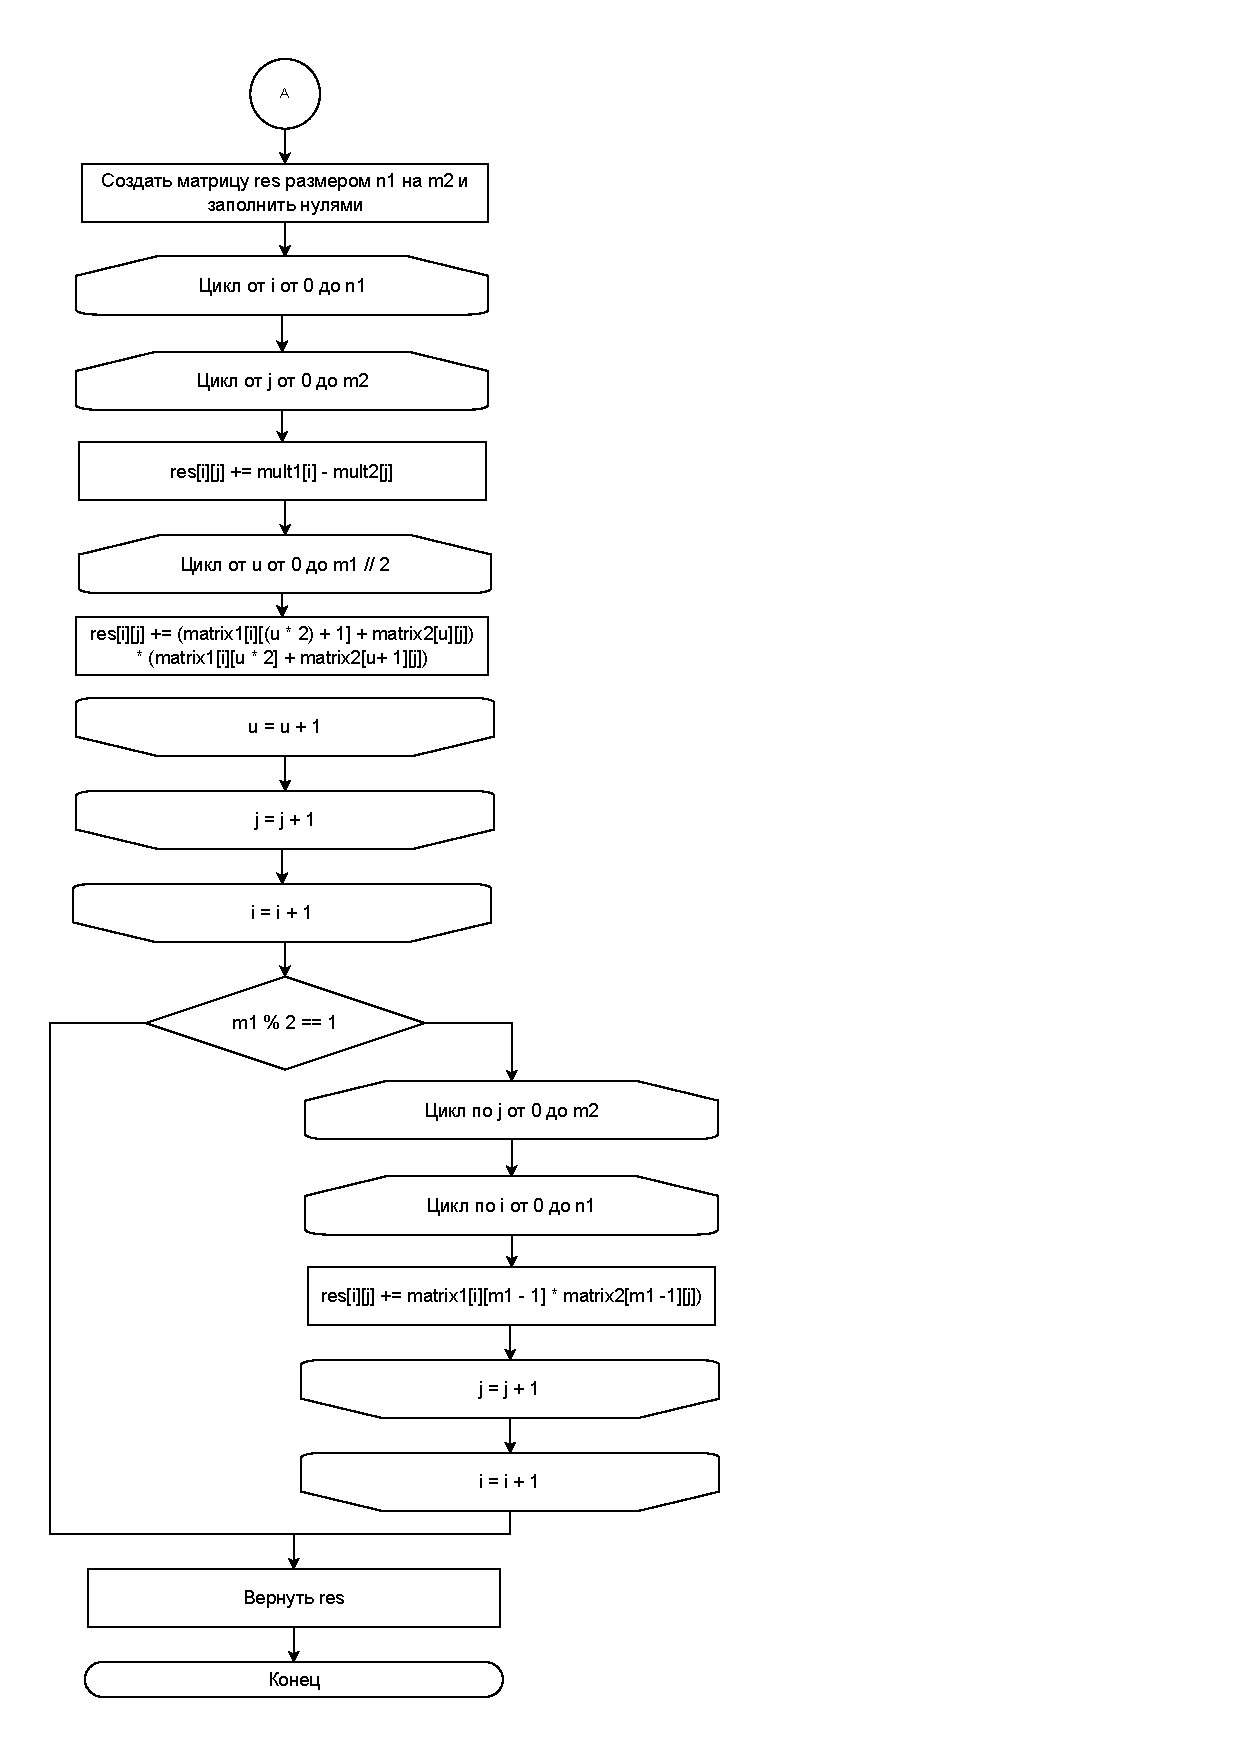
\includegraphics{img/win_12.pdf}}
    \caption{Алгоритм Винограда, часть 2.}
    \label{fig:win_12}
\end{figure}

\clearpage

\begin{figure}[H]
    \centering
    \adjustbox{scale=0.8, center}{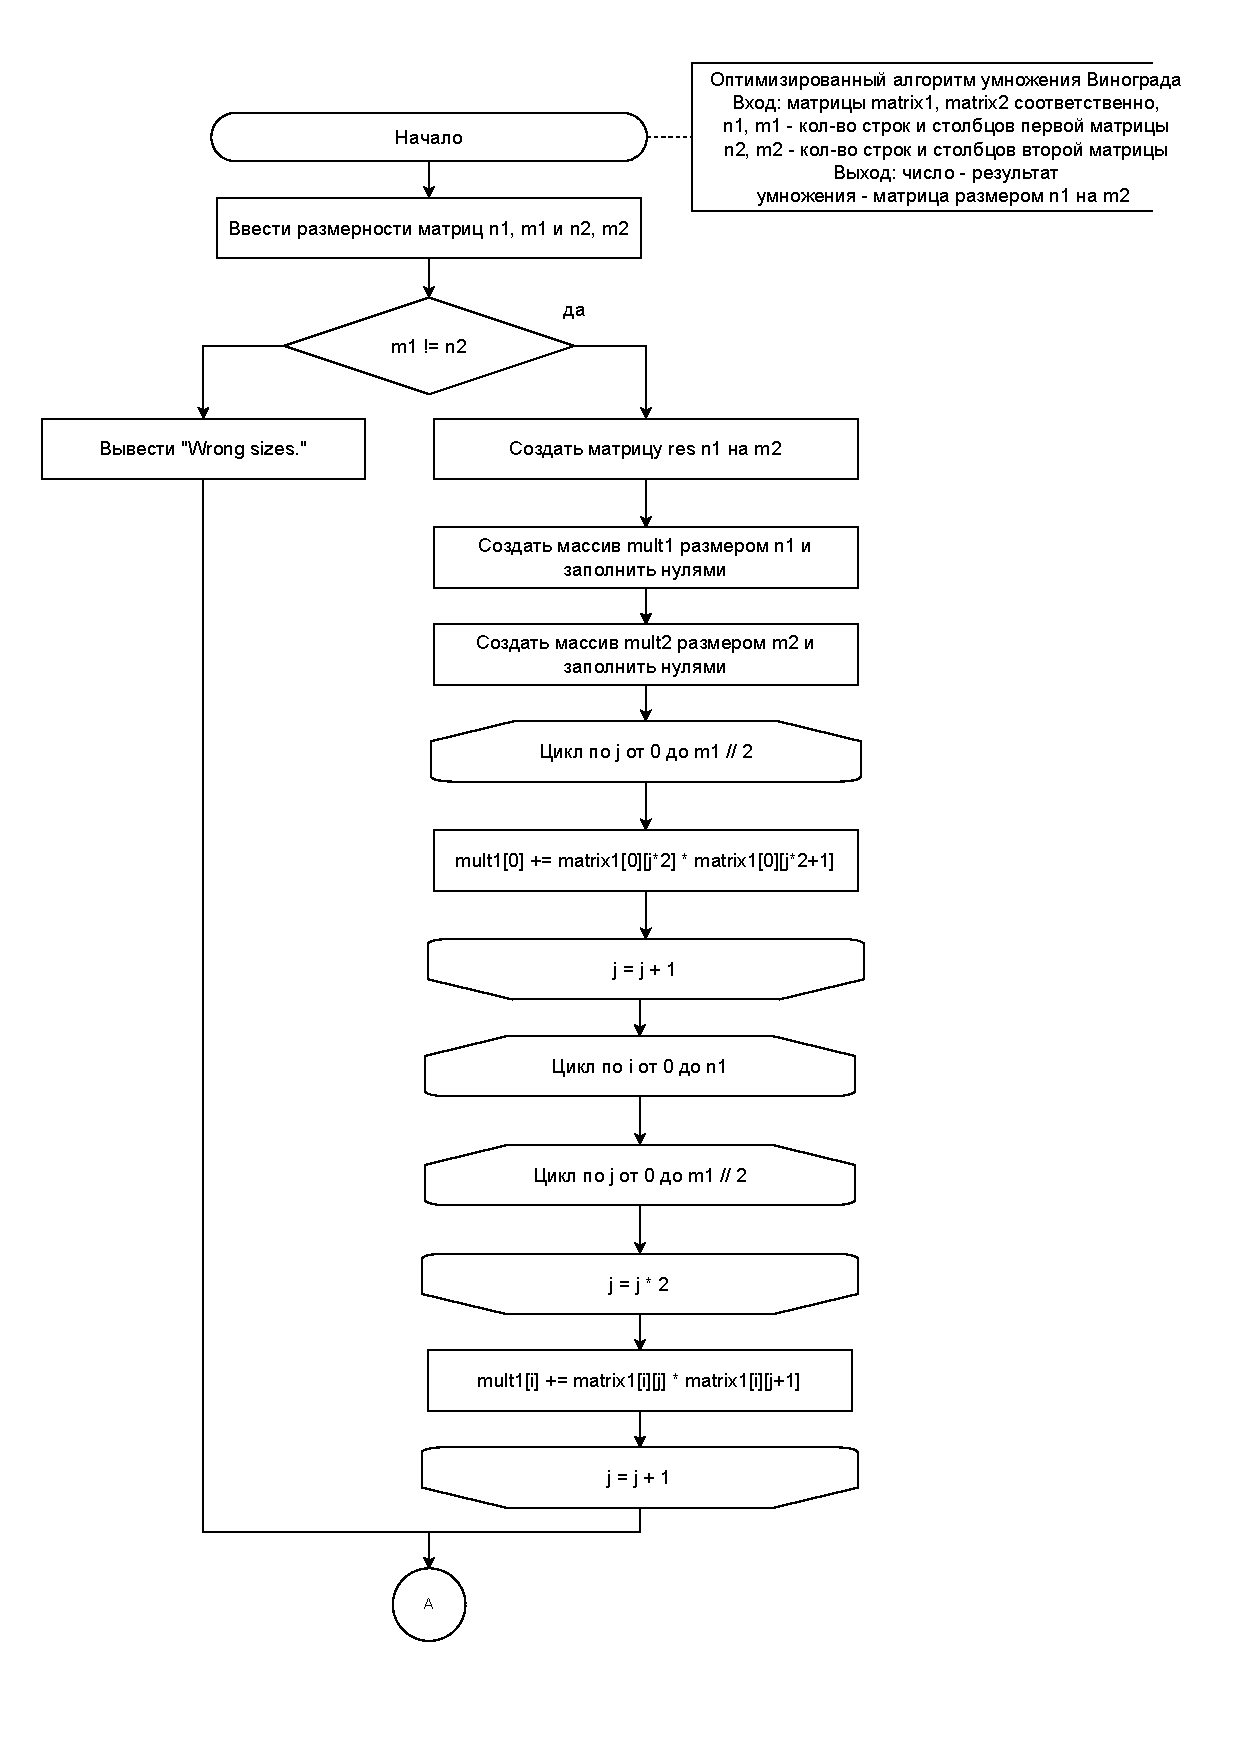
\includegraphics{img/win_21.pdf}}
    \caption{Оптимизированный алгоритм Винограда, часть 1.}
    \label{fig:win_21}
\end{figure}

\clearpage

\begin{figure}[H]
    \centering
    \adjustbox{scale=0.4, center}{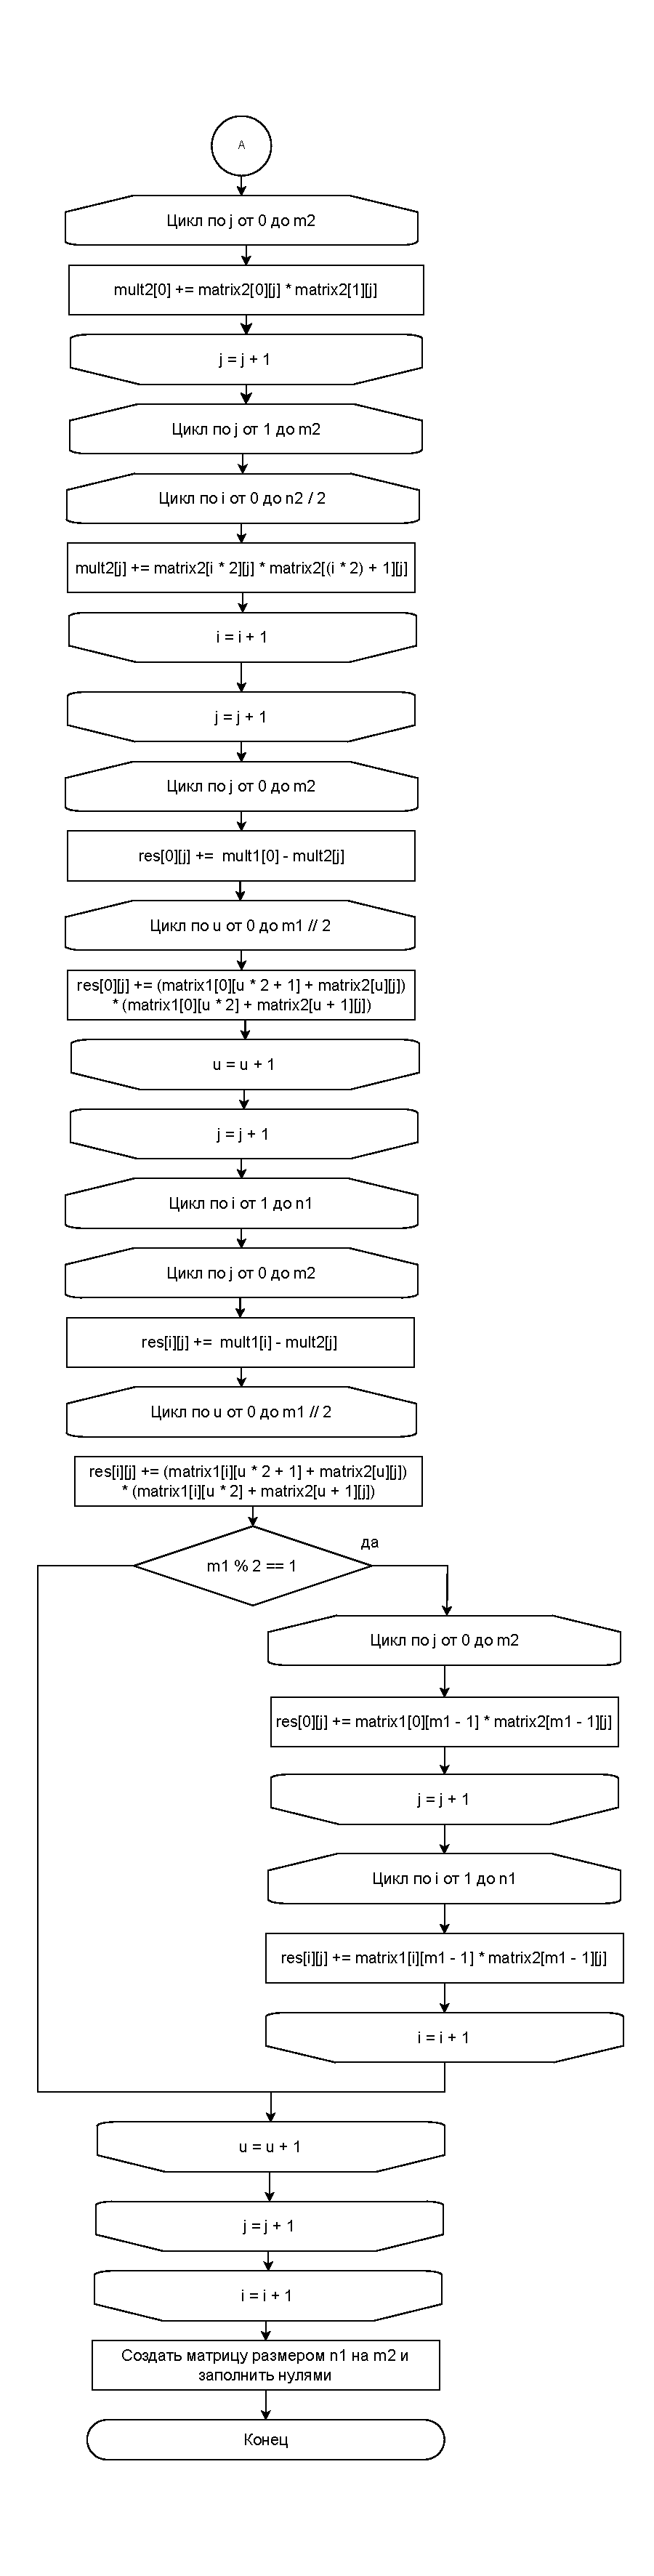
\includegraphics{img/win_22.pdf}}
    \caption{Оптимизированный алгоритм Винограда, часть 2.}
    \label{fig:win_22}
\end{figure}

\clearpage


\section{Модель вычисления трудоёмкости}

Для оценки трудоёмкости алгоритмов предложена модель, в которой трудоёмкость операций определяется следующим образом:

\begin{enumerate}
    \item[--] Операции типа \texttt{+, -=, +=, ==, !=, <, >, <=, >=, [], ++, --, \&\&, >>, <<, ||, \&, |} считаются с трудоёмкостью 1;
    
    \item[--] Операции \texttt{*, /, \%, *=, /=, \%=} имеют трудоёмкость 2;

    \item[--] Трудоёмкость выполнения условного оператора рассчитывается по следующей формуле~(\ref{eq:if}):
    \begin{equation}
    \label{eq:if}
    f_{\text{if}} = f_{\text{условия}} + 
    \begin{cases}
      \min(f_1, f_2), & \text{лучший случай},\\
      \max(f_1, f_2), & \text{иначе}.
    \end{cases}
    \end{equation}
    
    \item[--] Трудоёмкость выполнения цикла определяется по формуле~(\ref{eq:for}):
    \begin{equation}
    \label{eq:for}
    \begin{gathered}
      f_{\text{for}} = f_{\text{инициализация}} + f_{\text{сравнение}} +\\
      + M_{\text{итераций}} \cdot (f_{\text{тело цикла}} + f_{\text{инкремент}} + f_{\text{сравнение}})
    \end{gathered}
    \end{equation}

    \item[--] Трудоёмкость передачи аргументов в функцию и возврат из функции принимаются равными нулю.
\end{enumerate}

\section{Трудоёмкость алгоритма умножения матриц}

Необходимо рассмотреть трудоёмкость стандартного алгоритма умножения матриц.

\subsection{Инициализация результирующей матрицы}

Трудоёмкость инициализации матрицы, в которую записывается результат, вычисляется по следующей формуле:
\begin{equation}
f_{\text{иниц. матрицы}} = 2 + m_1 \cdot (2 + f_{n_2}) = 2 + m_1 \cdot (4 + n_2 \cdot 3) = 2 + 4 \cdot m_1 + 3 \cdot m_1 \cdot n_2,
\end{equation}
где $m_1$ — количество строк, $n_2$ — количество столбцов результирующей матрицы.

\subsection{Трудоёмкость стандартного алгоритма умножения матриц}

Трудоёмкость самого умножения. Внешний цикл по $i$ даёт следующий вклад:
\begin{equation}
f_{\text{умнож.}} = 2 + m_1 \cdot (f_i + 2) = 2 + m_1 \cdot (2 + n_2 \cdot (2 + f_j) + 2)
\end{equation}
С учётом всех вложенных циклов:
\begin{equation}
f_{\text{умнож.}} = 2 + m_1 \cdot (2 + n_2 \cdot (2 + 2 + n_1 \cdot (2 + f_k)) + 2)
\end{equation}
Итоговая трудоёмкость умножения вычисляется следующим образом:
\begin{equation}
f_{\text{умнож.}} = 2 + 4 \cdot m_1 + 4 \cdot m_1 \cdot n_2 + 10 \cdot m_1 \cdot n_1 \cdot n_2 \approx 10 \cdot m_1 \cdot n_1 \cdot n_2
\end{equation}

\subsection{Общая трудоёмкость}

Общая трудоёмкость алгоритма, включая инициализацию, рассчитывается по формуле:
\begin{equation}
f_{\text{общ.}} = 10 \cdot m_1 \cdot n_1 \cdot n_2 + 2 \cdot m_1 \cdot m_2 + 3 \cdot m_1 \cdot n_2 + 6 \cdot m_1 + 4 \approx 10 \cdot m_1 \cdot n_1 \cdot n_2
\end{equation}

\section{Трудоёмкость алгоритма Винограда умножения матриц}

Трудоёмкость алгоритма Винограда для умножения матриц состоит из нескольких частей:

\begin{enumerate}
    \item[--] создание массивов $mult1$ и $mult2$:
    \begin{equation}
    f_{mult1} = 3 \cdot n1 + 3 \cdot m1 + 4 \approx 3 \cdot n1 + 3 \cdot m1
    \end{equation}
    \begin{equation}
    f_{mult2} = 3 \cdot n2 + 3 \cdot m2 + 4 \approx 3 \cdot n2 + 3 \cdot m2
    \end{equation}

    \item[--] заполнение массивов $mult1$ и $mult2$:
    \begin{equation}
    f_{mult1} = 2 + n1 \cdot (2 + \lfloor m1 / 2 \rfloor) \approx 6.5 \cdot n1 \cdot \lfloor m1 / 2 \rfloor
    \end{equation}
    \begin{equation}
    f_{mult2} = 2 + n2 \cdot (2 + \lfloor m2 / 2 \rfloor) \approx 6.5 \cdot n2 \cdot \lfloor m2 / 2 \rfloor
    \end{equation}

    \item[--] инициализация матрицы--результата $res$:
    \begin{equation}
    f_{res} = m2 \cdot n1
    \end{equation}

    \item[--] заполнение матрицы для чётных индексов:
    \begin{equation}
    f_{even} = 2 + n1 \cdot \left(2 + m2 \cdot \left(6 + 2 + \lfloor m1 / 2 \rfloor\right)\right) \approx 11.5 \cdot n1 \cdot m2 \cdot \left\lfloor \frac{m1}{2} \right\rfloor
    \end{equation}

    \item[--] дополнительный цикл для нечётных индексов:
    \begin{equation}
    f_{odd} = 
    \begin{cases}
    2, & \text{если } m1 \text{ чётное} \\
    4 + 4 \cdot n1 + 12 \cdot n1 \cdot m2, & \text{иначе}
    \end{cases}
    \end{equation}
\end{enumerate}

Таким образом, трудоёмкость алгоритма Винограда в лучшем случае равна:
\begin{equation}
f_{best} \approx 11.5 \cdot n1 \cdot m2 \cdot \left\lfloor \frac{m1}{2} \right\rfloor
\end{equation}

Трудоёмкость в худшем случае выражается следующим образом:
\begin{equation}
f_{\text{worst}} = 3 \cdot n_1 + 3 \cdot m_1 + 6.5 \cdot n_1 \cdot \left\lfloor \frac{m_1}{2} \right\rfloor + 6.5 \cdot n_2 \cdot \left\lfloor \frac{m_2}{2} \right\rfloor 
+ m_2 \cdot n_1 + 11.5 \cdot n_1 \cdot m_2 + 4 + 4 \cdot n_1 + 12 \cdot n_1 \cdot m_2
\end{equation}

Или:
\begin{equation}
f_{worst} \approx 11.5 \cdot n1 \cdot m2 + 3 \cdot n1 + 3 \cdot m1 + 6.5 \cdot n2 \cdot \left\lfloor \frac{m2}{2} \right\rfloor + 4
\end{equation}

\section{Трудоёмкость оптимизированного алгоритма Винограда умножения матриц}

\subsection{Оптимизации в алгоритме}
В данном задании, согласно варианту, предусмотрены следующие дополнительные оптимизации:

\begin{itemize}
    \item[--] использование двоичного сдвига вместо умножения на 2, что позволяет выполнять вычисления быстрее на уровне процессора;
    \item[--] объединение III и IV частей алгоритма Винограда для повышения эффективности по времени;
    \item[--] вынос начальной итерации из внешних циклов, что сокращает количество операций внутри циклов и ускоряет выполнение программы.
\end{itemize}

\section{Трудоёмкость оптимизированного алгоритма Винограда умножения матриц}

\subsection{Оптимизации в алгоритме}
В данном задании, согласно варианту, предусмотрены следующие дополнительные оптимизации:

\begin{itemize}
    \item[--] использование двоичного сдвига вместо умножения на 2, что позволяет выполнять вычисления быстрее на уровне процессора;
    \item[--] объединение III и IV частей алгоритма Винограда для повышения эффективности по времени;
    \item[--] вынос начальной итерации из внешних циклов, что сокращает количество операций внутри циклов и ускоряет выполнение программы.
\end{itemize}

\subsection{Трудоёмкость оптимизированного алгоритма Винограда}

Трудоёмкость алгоритма Винограда для умножения матриц состоит из нескольких компонентов:

\begin{itemize}
    \item[--] создание массивов $mult1$ и $mult2$:
    \begin{equation}
    f = f_{mult1} + f_{mult2} = 3 \cdot m_1 + 3 \cdot n_2 + 4 \approx 3 \cdot m_1 + 3 \cdot n_2
    \end{equation}

    \item[--] заполнение $mult1$ и $mult2$:
    \begin{equation}
    f_{mult1} \approx 5 \cdot m_1 \cdot n_1
    \end{equation}
    \begin{equation}
    f_{mult2} \approx 5 \cdot n_2 \cdot m_2
    \end{equation}

    \item[--] инициализация матрицы-результата:
    \begin{equation}
    f \approx n_2 \cdot m_1
    \end{equation}

    \item[--] цикл заполнения для чётных:
    \begin{equation}
    f = 9 \cdot n_1 \cdot n_2 \cdot m_1
    \end{equation}
\end{itemize}

Таким образом, трудоёмкость в лучшем случае может быть выражена как:
\begin{equation}
f_{\text{лучший}} \approx 9 \cdot n_1 \cdot n_2 \cdot m_1
\end{equation}

В худшем случае трудоёмкость аналогична:
\begin{equation}
f_{\text{худший}} \approx 9 \cdot n_1 \cdot n_2 \cdot m_1
\end{equation}

Итоговая трудоёмкость:
\begin{equation}
f_{\text{итог}} \approx 9 \cdot n_1 \cdot n_2 \cdot m_1
\end{equation}

Таким образом, оптимизированный алгоритм Винограда имеет трудоёмкостью, приблизительно равной $9 \cdot n_1 \cdot n_2 \cdot m_1$.

\section*{Вывод}
В данном разделе разработаны описания алгоритмов умножения матриц, а также рассмотрены основные параметры для оценки их трудоёмкости. Описаны структуры данных, взаимодействие пользователя с программой, а также проведена теоретическая оценка трудоёмкости классического алгоритма умножения матриц, алгоритма Винограда и его оптимизированной версии.


\chapter{Технологическая часть}
В данном разделе приведены данные о выбранном языке программирования, реализации алгоритмов и тесты для каждого алгоритма.

\section{Требования к программному обеспечению}
Для корректной работы программного обеспечения предусмотрены следующие требования:
\begin{itemize}
    \item[--] Входные данные: две матрицы $matrix1$ и $matrix2$. Количество столбцов в матрице $matrix1$ должно совпадать с количеством строк в матрице $matrix2$.
    \item[--] Выходные данные: результат умножения входных матриц, представленный в матрице $result\_matrix$.
\end{itemize}

\section{Средства реализации}
Для реализации алгоритмов, проведения замеров времени и построения графиков используется язык программирования \texttt{Python}~\cite{bib3}. \texttt{Python} предоставляет все необходимые инструменты для реализации матричных алгоритмов и построения графиков. В ходе разработки алгоритмов применяются следующие типы и структуры данных:
\begin{itemize} 
    \item[--] двумерные матрицы типа \texttt{int}; 
    \item[--] переменные для хранения количества строк и столбцов в матрицах. 
\end{itemize}

Замеры времени выполняются с помощью функции \texttt{process\_time}~\cite{bib4}.


\section{Структура программы}
Программа состоит из нескольких модулей: 
\begin{itemize}
    \item[--] \texttt{main.py} -- файл, который обеспечивает интерфейс и взаимодействие с пользователем, а также выполняет замеры времени работы алгоритмов; 
    \item[--] \texttt{algs.py} -- файл, содержащий реализацию всех алгоритмов; 
    \item[--] \texttt{in\_out.py} -- модуль для ввода и вывода данных; 
    \item[--] \texttt{compare\_time.py} -- модуль для сравнения времени выполнения алгоритмов.
\end{itemize}

\section{Реализация алгоритмов}

В листинге~\ref{lst:create_matrix} представлена реализация функции \texttt{insert\_matrix}, которая создаёт матрицу, запрашивая ввод элементов с клавиатуры.
\begin{center}
\captionsetup{justification=raggedright,singlelinecheck=off}
\begin{lstlisting}
def insert_matrix(n: int, m: int):
    matrix = [[0 for _ in range(m)] for _ in range(n)]
    for i in range(n):
        for j in range(m):
            matrix[i][j] = int(input())
    return matrix
\end{lstlisting}
\captionsetup{justification=centering, singlelinecheck=off}
\captionof{lstlisting}{Реализация создания матрицы через ввод с клавиатуры}
\label{lst:create_matrix}
\end{center}

В листинге~\ref{lst:create_random_matrix} представлена реализация функции \texttt{create\_random\_matrix}, которая генерирует случайную матрицу с элементами от 0 до 100.
\begin{center}
\captionsetup{justification=raggedright,singlelinecheck=off}
\begin{lstlisting}
def create_random_matrix(n: int, m: int):
    matrix = [[random.randint(0, 100) for _ in range(m)] for _ in range(n)]  
    return matrix
\end{lstlisting}
\captionsetup{justification=centering, singlelinecheck=off}
\captionof{lstlisting}{Реализация генерации случайной матрицы с элементами от 0 до 100}
\label{lst:create_random_matrix}
\end{center}

В листинге~\ref{lst:print_answer} представлена реализация функции \texttt{print\_answer}, которая выводит матрицу на экран.
\begin{center}
\captionsetup{justification=raggedright,singlelinecheck=off}
\begin{lstlisting}
def print_answer(matrix, verbose=True):
    if not verbose:
        return  
    for i, row in enumerate(matrix):
        print("  " + " ".join(f"{val:2}" for val in row)) 
\end{lstlisting}
\captionsetup{justification=centering, singlelinecheck=off}
\captionof{lstlisting}{Реализация вывода матрицы}
\label{lst:print_answer}
\end{center}

В листинге~\ref{lst:multiply_base} представлена реализация функции \texttt{multiply\_base}, которая выполняет умножение матриц с использованием стандартного алгоритма.
\begin{center}
\captionsetup{justification=raggedright,singlelinecheck=off}
\begin{lstlisting}
def multiply_base(matrix1, matrix2):
    n1 = len(matrix1)
    m1 = len(matrix1[0])
    n2 = len(matrix2)
    m2 = len(matrix2[0])

    if m1 != n2:
        print("Wrong sizes.")
        return []
        
    res = [[0] * m2 for _ in range(n1)]
    
    for i in range(n1):
        for j in range(m2):
            for u in range(m1):
                res[i][j] += matrix1[i][u] * matrix2[u][j]
    return res
\end{lstlisting}
\captionsetup{justification=centering, singlelinecheck=off}
\captionof{lstlisting}{Реализация умножения матриц с использованием стандартного алгоритма}
\label{lst:multiply_base}
\end{center}

В листинге~\ref{lst:multiply_win} представлена реализация функции \texttt{multiply\_win}, которая выполняет умножение матриц с использованием алгоритма Винограда.
\begin{center}
\captionsetup{justification=raggedright,singlelinecheck=off}
\begin{lstlisting}
def multiply_win(matrix1, matrix2):
    n1 = len(matrix1)
    m1 = len(matrix1[0])
    n2 = len(matrix2)
    m2 = len(matrix2[0])

    if m1 != n2:
        print("Wrong sizes.")
        return []
    res = [[0] * m2 for _ in range(n1)]
    mult1 = [0] * n1
    for j in range(m1 // 2):
        mult1[0] += matrix1[0][j * 2] * matrix1[0][(j * 2) + 1]
    for i in range(1, n1, 1):
        for j in range(m1 // 2):
            mult1[i] += matrix1[i][j * 2] * matrix1[i][(j * 2) + 1]

    mult2 = [0] * m2
    for i in range(n2 // 2):
        mult2[0] += matrix2[i * 2][0] * matrix2[(i * 2) + 1][0]
    for j in range(1, m2, 1):
        for i in range(n2 // 2):
            mult2[j] += matrix2[i * 2][j] * matrix2[(i * 2) + 1][j]

    for j in range(m2):
        res[0][j] = mult1[0] - mult2[j]
        for u in range(m1 // 2):
            res[0][j] += (matrix1[0][(u * 2) + 1] + matrix2[u][j]) * \
                                  (matrix1[0][u * 2] + matrix2[u + 1][j])
    for i in range (1, n1, 1):
        for j in range(m2):
            res[i][j] = mult1[i] - mult2[j]
            for u in range(m1 // 2):
                res[i][j] += (matrix1[i][(u * 2) + 1] + matrix2[u][j]) * \
                                  (matrix1[i][u * 2] + matrix2[u + 1][j])
    if m1 % 2 == 1:
        for j in range(m2):
            res[0][j] += matrix1[0][m1 - 1] * matrix2[m1 - 1][j]
        for i in range(1, n1, 1):
            for j in range(m2):
                res[i][j] += matrix1[i][m1 - 1] * matrix2[m1 - 1][j]
    return res
\end{lstlisting}
\captionsetup{justification=centering, singlelinecheck=off}
\captionof{lstlisting}{Реализация умножения матриц с использованием алгоритма Винограда}
\label{lst:multiply_win}
\end{center}


В листинге~\ref{lst:multiply_winograd_optimized} представлена реализация функции \texttt{multiply\_win\_op}, которая выполняет умножение матриц, используя оптимизированный алгоритм Винограда.

\begin{lstlisting}
def multiply_win_op(matrix1, matrix2):

    n1 = len(matrix1)
    m1 = len(matrix1[0])
    n2 = len(matrix2)
    m2 = len(matrix2[0])

    if m1 != n2:
        print("Wrong sizes.")
        return []
    
    res = [[0] * m2 for _ in range(n1)]

    mult1 = [0] * n1
    for j in range(m1 >> 1):
        mult1[0] += matrix1[0][j << 1] * matrix1[0][(j << 1) + 1]
    for i in range(1, n1):
        for j in range(m1 >> 1):
            mult1[i] += matrix1[i][j << 1] * matrix1[i][(j << 1) + 1]
            
    mult2 = [0] * m2
    for i in range(n2 >> 1):
        mult2[0] += matrix2[i << 1][0] * matrix2[(i << 1) + 1][0]
    for j in range(1, m2):
        for i in range(n2 >> 1):
            mult2[j] += matrix2[i << 1][j] * matrix2[(i << 1) + 1][j]

    for j in range(m2):
        res[0][j] = mult1[0] - mult2[j]
        for u in range(m1 >> 1):
            res[0][j] += (matrix1[0][(u << 1) + 1] + matrix2[u][j]) * \
                                  (matrix1[0][u << 1] + matrix2[u + 1][j])
    for i in range(1, n1):
        for j in range(m2):
            res[i][j] = mult1[i] - mult2[j]
            for u in range(m1 >> 1):
                res[i][j] += (matrix1[i][(u << 1) + 1] + matrix2[u][j]) * \
                                  (matrix1[i][u << 1] + matrix2[u + 1][j])
    if m1 % 2 == 1:
        for j in range(m2):
            res[0][j] += matrix1[0][m1 - 1] * matrix2[m1 - 1][j]
        for i in range(1, n1):
            for j in range(m2):
                res[i][j] += matrix1[i][m1 - 1] * matrix2[m1 - 1][j]
    return res
\end{lstlisting}
\captionsetup{justification=centering, singlelinecheck=off}
\captionof{lstlisting}{Реализация умножения матриц с использованием оптимизированного алгоритма Винограда}
\label{lst:multiply_winograd_optimized}
\clearpage

\section{Функциональные тесты}
В таблице~\ref{tbl:functional_test} приведены результаты функционального тестирования для алгоритмов, реализующих умножение матриц. Все тесты пройдены успешно.

\begin{table}[h]
    \begin{center}
        \begin{threeparttable}
            \captionsetup{justification=raggedright,singlelinecheck=off}
            \begin{tabular}{|c|c|c|c|}
                \hline
                \textbf{1-ая матрица} & \textbf{2-ая матрица} & \textbf{Ожидаемый результат} & \textbf{Фактический результат} \\ \hline
                $\begin{pmatrix}
                    1 & 2 \\
                    3 & 4
                \end{pmatrix}$ & 
                $\begin{pmatrix}
                    5 & 6 \\
                    7 & 8
                \end{pmatrix}$ & 
                $\begin{pmatrix}
                    19 & 22 \\
                    43 & 50
                \end{pmatrix}$ & 
                $\begin{pmatrix}
                    19 & 22 \\
                    43 & 50
                \end{pmatrix}$ \\ \hline
                
                $\begin{pmatrix}
                    1 & 2 & 3
                \end{pmatrix}$ & 
                $\begin{pmatrix}
                    4 \\
                    5 \\
                    6
                \end{pmatrix}$ & 
                $\begin{pmatrix}
                    32
                \end{pmatrix}$ & 
                $\begin{pmatrix}
                    32
                \end{pmatrix}$ \\ \hline
                
                $\begin{pmatrix}
                    2 & 0 \\
                    1 & 2
                \end{pmatrix}$ & 
                $\begin{pmatrix}
                    1 & 3 \\
                    4 & 0
                \end{pmatrix}$ & 
                $\begin{pmatrix}
                    14 & 6 \\
                    10 & 6
                \end{pmatrix}$ & 
                $\begin{pmatrix}
                    14 & 6 \\
                    10 & 6
                \end{pmatrix}$ \\ \hline
                
                $\begin{pmatrix}
                    1 & 2 & 3
                \end{pmatrix}$ & 
                $\begin{pmatrix}
                    0 \\
                    0 \\
                    0
                \end{pmatrix}$ & 
                $\begin{pmatrix}
                    0
                \end{pmatrix}$ & 
                $\begin{pmatrix}
                    0
                \end{pmatrix}$ \\ \hline
                
                $\begin{pmatrix}
                    0 & 0
                \end{pmatrix}$ & 
                $\begin{pmatrix}
                    0 & 0
                \end{pmatrix}$ & 
                $\begin{pmatrix}
                    0
                \end{pmatrix}$ & 
                $\begin{pmatrix}
                    0
                \end{pmatrix}$ \\ \hline
                
                $\begin{pmatrix}
                    3 & 1 \\
                    2 & 4
                \end{pmatrix}$ & 
                $\begin{pmatrix}
                    2 & 3 \\
                    1 & 0
                \end{pmatrix}$ & 
                $\begin{pmatrix}
                    9 & 18 \\
                    10 & 14
                \end{pmatrix}$ & 
                $\begin{pmatrix}
                    9 & 18 \\
                    10 & 14
                \end{pmatrix}$ \\ \hline
            \end{tabular}
        \end{threeparttable}
    \end{center}
    \caption{\label{tbl:functional_test} Функциональные тесты}
\end{table}


\section*{Вывод}
В данном разделе представлены результаты тестирования алгоритмов умножения матриц. Все тесты прошли успешно, фактические результаты совпадают с ожидаемыми. Алгоритмы корректно обрабатывают ошибки при несовпадении размеров матриц. 


\chapter{Исследовательская часть}
В данном разделе представлены результаты исследования эффективности работы алгоритмов по времени выполнения, основанной на критерии временных затрат.

\section{Технические характеристики}
Технические характеристики компьютера, на котором проводились замеры времени:

\begin{itemize} 
    \item[--] операционная система: macOS Monterey;
    \item[--] оперативная память: 8 ГБ;
    \item[--] процессор: Quad-Core Intel Core i5 с тактовой частотой 1.4 ГГц;
\end{itemize}

\section{Сравнительный анализ времени выполнения алгоритмов}
\justifying

Замеры проводились на матрицах размерностью от 20 до 100. Выбор размерностей обусловлен необходимостью анализа производительности алгоритмов на различных уровнях сложности, что выявляет их особенности и характеристики. Для достижения высокой точности полученных данных было выполнено по 100 замеров для каждой размерности.
Результаты замеров представлены в таблицах~\ref{tbl:time_table_1} и~\ref{tbl:time_table_2}. На рисунках~\ref{fig:even_graph} и~\ref{fig:odd_graph} отображены графики, построенные на основе табличных данных.

\begin{table}[h]
    \centering
    \begin{adjustbox}{max width=\textwidth} 
    \begin{tabular}{|r|r|r|r|} 
    \hline
    Размер & Классический & Виноград & Оптимизированный Виноград \\ 
    \hline
    20    & 2.14e-03    & 2.46e-03 & 2.78e-03 \\ \hline
    30    & 7.12e-03    & 9.41e-03 & 9.04e-03 \\ \hline
    40    & 1.71e-02    & 1.83e-02 & 2.13e-02 \\ \hline
    50    & 3.33e-02    & 3.58e-02 & 4.15e-02 \\ \hline
    60    & 6.00e-02    & 6.00e-02 & 7.20e-02 \\ \hline
    70    & 9.24e-02    & 9.38e-02 & 1.12e-01 \\ \hline
    80    & 1.37e-01    & 1.42e-01 & 1.66e-01 \\ \hline
    \end{tabular}
    \end{adjustbox}
    \caption{Результаты измерений времени выполнения алгоритмов при чётной размерности матриц (в секундах).}
    \label{tbl:time_table_1}
\end{table}

\begin{table}[h]
    \centering
    \begin{adjustbox}{max width=\textwidth} 
    \begin{tabular}{|r|r|r|r|} 
    \hline
    Размер & Классический & Виноград & Оптимизированный Виноград \\ 
    \hline
    19    & 1.95e-03    & 2.14e-03 & 3.12e-03 \\ \hline
    29    & 7.24e-03    & 7.06e-03 & 8.26e-03 \\ \hline
    39    & 2.13e-02    & 1.90e-02 & 1.94e-02 \\ \hline
    49    & 3.04e-02    & 3.23e-02 & 3.76e-02 \\ \hline
    59    & 5.30e-02    & 5.60e-02 & 6.55e-02 \\ \hline
    79    & 1.26e-01    & 1.32e-01 & 1.60e-01 \\ \hline
    89    & 1.80e-01    & 1.92e-01 & 2.25e-01 \\ \hline
    99    & 2.47e-01    & 2.57e-01 & 3.02e-01 \\ \hline
    \end{tabular}
    \end{adjustbox}
    \caption{Результаты измерений времени выполнения алгоритмов при нечётной размерности матриц (в секундах).}
    \label{tbl:time_table_2}
\end{table}

\begin{figure}[h]
    \centering
    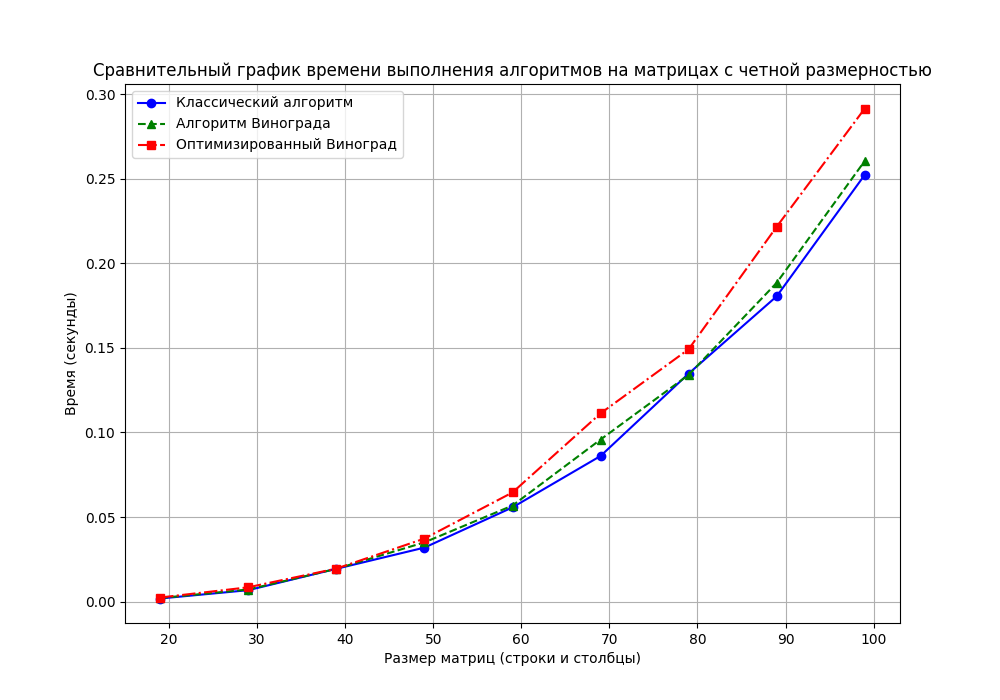
\includegraphics[scale=0.6]{img/even.png}
    \caption{Сравнительный график времени выполнения алгоритмов на матрицах с чётной размерностью.}
    \label{fig:even_graph}
\end{figure}

\begin{figure}[h]
    \centering
    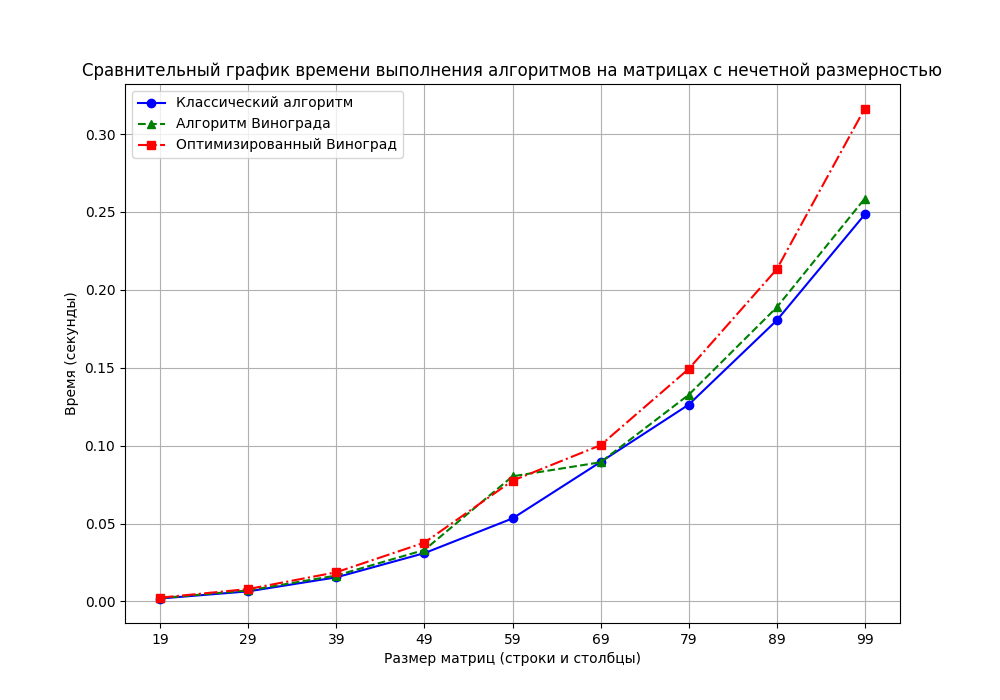
\includegraphics[scale=0.6]{img/odd.png}
    \caption{Сравнительный график времени выполнения алгоритмов на матрицах с нечётной размерностью.}
    \label{fig:odd_graph}
\end{figure}
\clearpage

\newpage
\section*{Вывод}
Стандартный алгоритм и алгоритм Винограда демонстрируют схожие временные затраты на матрицах размером до $300 \times 300$. Однако производительность алгоритма Винограда падает на больших размерностях (от $500 \times 500$). В отличие от них, оптимизированный алгоритм Винограда работает быстрее, и с увеличением размеров матриц разница в скорости становится более значимой.

Стандартный алгоритм Винограда показал себя менее эффективным, особенно на нечётных матрицах, где требуется больше дополнительных вычислений, в то время как оптимизированный алгоритм практически не теряет в скорости благодаря оптимизации.

Таким образом, оптимизированный алгоритм Винограда является самым быстрым решением для матриц размером (от $500 \times 500$). Стандартный алгоритм Винограда менее эффективен на нечётных матрицах из-за необходимости дополнительных вычислений. Классический алгоритм оказался самым медленным на матрицах от $500 \times 500$, но может быть полезен при решении небольших задач. Поэтому для оптимального умножения матриц предпочтителен оптимизированный алгоритм Винограда.
\clearpage


\chapter*{ЗАКЛЮЧЕНИЕ}
\addcontentsline{toc}{chapter}{ЗАКЛЮЧЕНИЕ}
Цель работы достигнута. В ходе выполнения данной лабораторной работы решены следующие задачи:
\begin{itemize}
    \item[--] реализованы и проанализированы классический алгоритм умножения матриц, алгоритм Винограда и его оптимизированная версия;
    \item[--] проведён анализ временных затрат алгоритмов умножения матриц на различных размерностях, что позволило выявить их особенности и различия в производительности;
    \item[--] выполнен анализ трудоёмкости алгоритмов, учитывающий количество операций и требования к памяти;
    \item[--] подготовлены графики, которые демонстрируют результаты сравнительного анализа;
    \item[--] разработаны тесты для проверки правильности и эффективности работы реализованных алгоритмов по критериям временных затрат и использования памяти;
    \item[--] представлены полученные результаты в виде отчёта о выполненной лабораторной работе.
\end{itemize}

Исследования показали, что оптимизированный алгоритм Винограда наиболее эффективен для умножения матриц размером от $500 \times 500$. Он быстрее алгоритма умножения матриц и стандартного алгоритма Винограда.

\renewcommand{\bibname}{СПИСОК ИСПОЛЬЗОВАННЫХ ИСТОЧНИКОВ}
\begin{thebibliography}{4}
    \bibitem{bib1}
    Голуб, Дж. \& Ван Лоун, Ч. Матричные вычисления: Пер. с англ. — М.: Мир, 1999. — 548 с., ил. — ISBN 5-03-002406-9.

    \bibitem{bib2}
    Coppersmith, D. \& Winograd, S. Matrix multiplication via arithmetic progressions. В: Proceedings of the nineteenth annual ACM symposium on Theory of computing. — New York: ACM, 1987. — С. 1–6.

    \bibitem{bib3}
    Python Software Foundation. Официальная документация по Python [Электронный ресурс]. — Режим доступа: \url{https://www.python.org/doc/} (дата обращения: 22.10.2024).

    \bibitem{bib4}
    Python Software Foundation. Модуль time — Доступ к времени и его преобразования [Электронный ресурс]. — Режим доступа: \url{https://docs.python.org/3/library/time.html} (дата обращения: 22.10.2024).
\end{thebibliography}


%\chapter*{СПИСОК ИСПОЛЬЗОВАННЫХ ИСТОЧНИКОВ}
\addcontentsline{toc}{chapter}{СПИСОК ИСПОЛЬЗОВАННЫХ ИСТОЧНИКОВ}

\end{document}